\subsection{home.web.cern.ch}

En este experimento se creo un paquete ICMP con dirección IP destino \textit{137.138.76.28}, correspondiente a la web \textit{http://home.web.cern.ch/} página oficial de la Organización Europea para la Investigación Nuclear (CERN). Los servidores de este sitio web se encuentran en la ciudad de Ginebra, Suiza. Se espera por lo tanto que a lo largo del camino que tome el paquete haya un salto transoceánico entre dos hops que obtendrá un alto puntaje según el z-score. Veamos primero una lista de las IPs junto a los lugares físicos asociados a esta para visualizar con mayor facilidad el recorrido que realizó el paquete a lo largo del experimento:

\begin{figure}[H]
  \centering	
	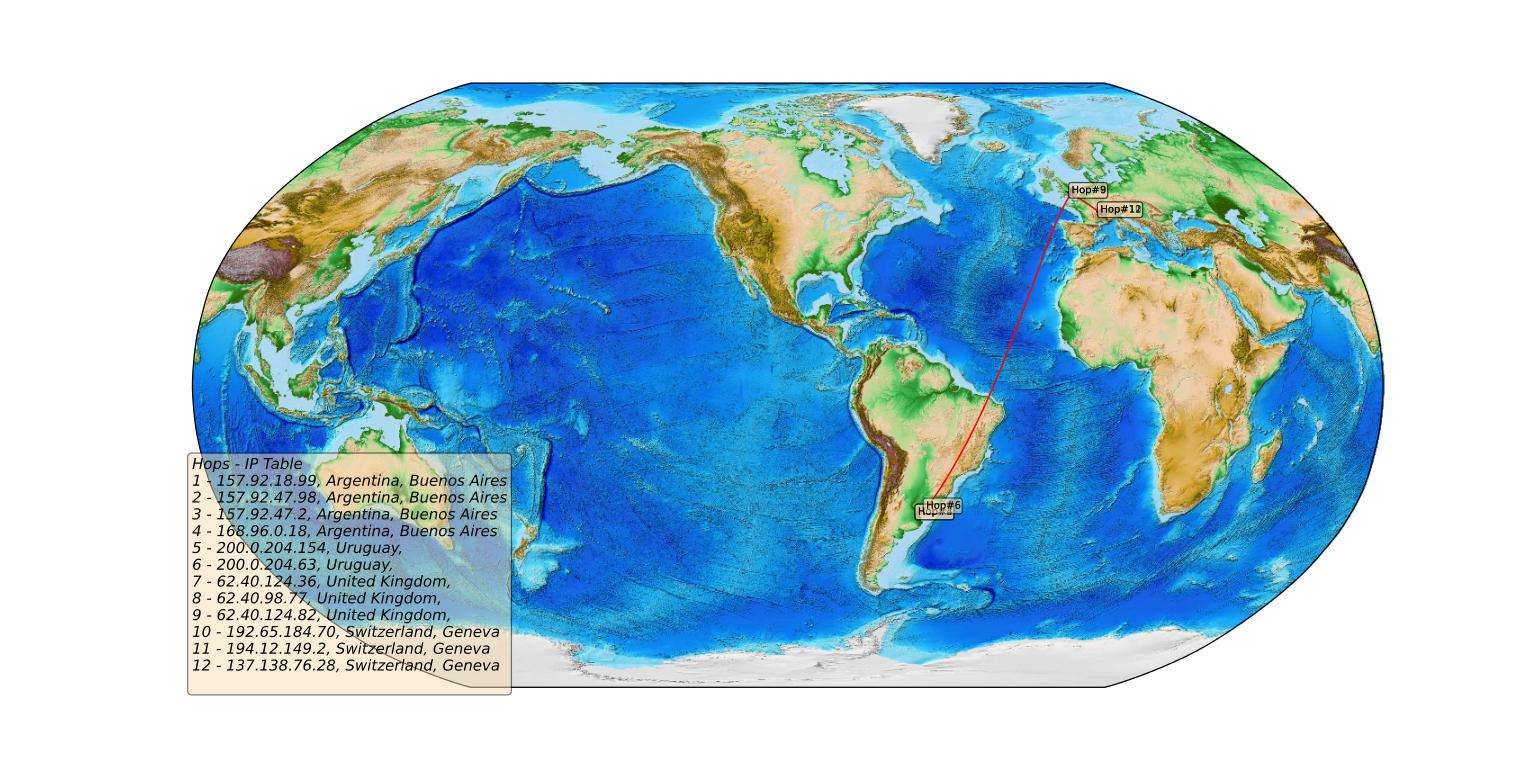
\includegraphics[scale=0.3]{../cern-experiment/figure_1.jpeg}
  \caption{Mapamundi con un croquis del viaje realizado por el paquete en rojo.}
	\label{fig:histo-src-sitiotrabajo}
\end{figure}

Como se puede ver el \textit{hop} entre el sexto y septimo hop es el transoceánico del que se habló anteriormente. El salto se produce entre Uruguay (\textit{200.0.204.63}) y el Reino Unido (\textit{62.40.124.36}). En el siguiente gráfico, que muestra el RTT entre dos hops consecutivos medido en milisegundos, el salto que arriba al Reino Unido es el que devuelve el valor más alto. Esto tiene sentido ya que este es el de mayor distancia geográfica.

\begin{figure}[H]
  \centering	
	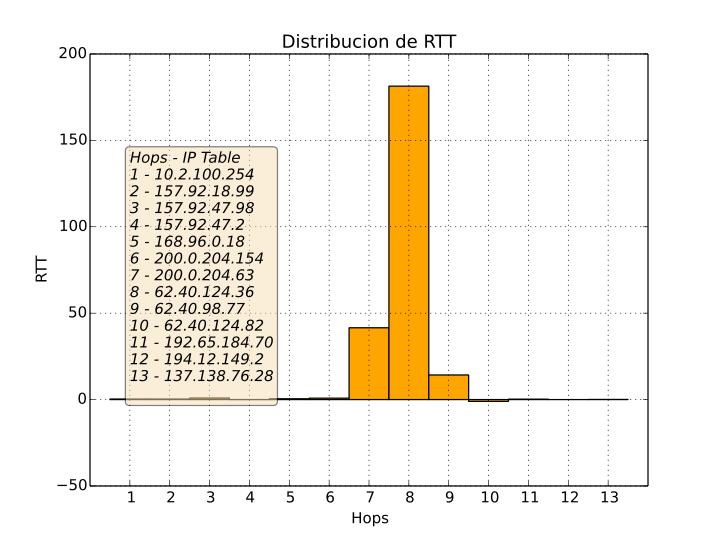
\includegraphics[scale=0.4]{../cern-experiment/bar_rtt.jpeg}
  \caption{RTT entre dos hop consecutivos medido en milisegundos.}
	\label{fig:histo-src-sitiotrabajo}
\end{figure}

\begin{figure}[H]
  \centering	
	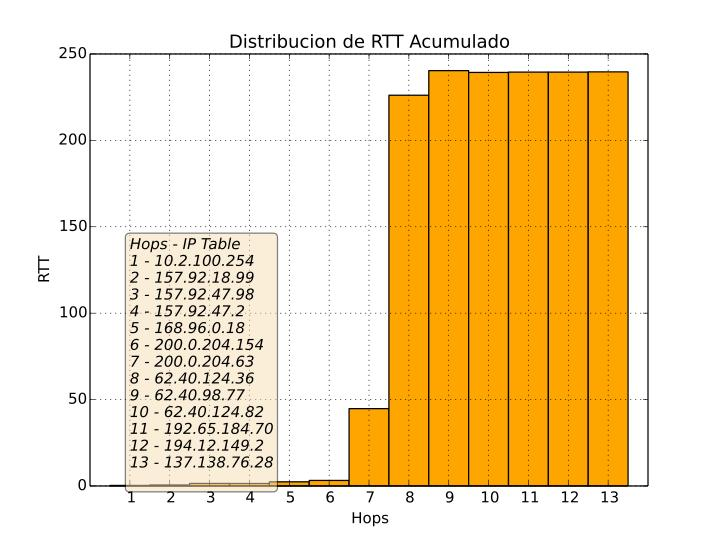
\includegraphics[scale=0.4]{../cern-experiment/bar_rtt_acum.jpeg}
  \caption{RTT acumulado del paquete a medida que avanza en su camino hacia el host del CERN.}
	\label{fig:histo-src-sitiotrabajo}
\end{figure}

Finalmente, se pueden ver los resultados obtenidos con el \textit{z-score} donde se observan valores similares (en proporción) a los obtenidos en el primer gráfico de esta sección. Más aun, el puntaje fue negativo para aquellos saltos que pueden ser etiquetados como de menor importancia, aquellos que tienen un desplazamiento geográfico menor y en consecuencia no aportan demasiado al tiempo total de viaje del paquete. Entre los saltos destacados, se puede ver una diferencia más pronunciada a la hora de encontrar al octavo como \textit{hop} distinguido.

\begin{figure}[H]
  \centering	
	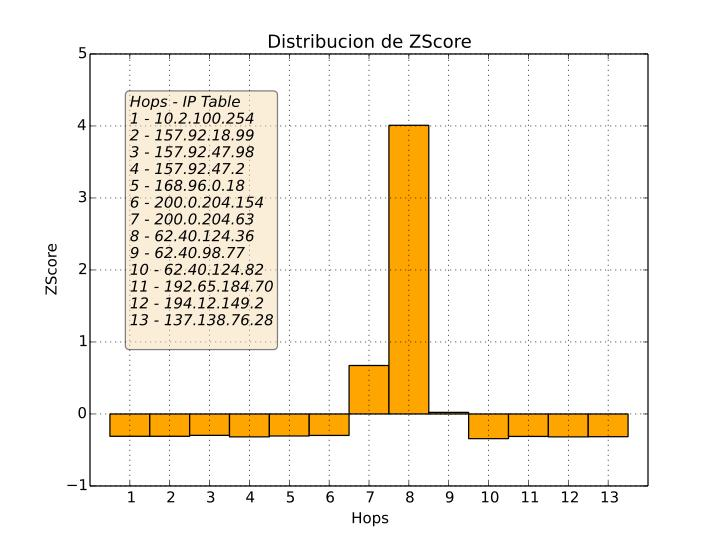
\includegraphics[scale=0.4]{../cern-experiment/bar_z_score.jpeg}
  \caption{Z-Score para cada uno de los saltos.}
	\label{fig:histo-src-sitiotrabajo}
\end{figure}


\subsubsection{Tabla de Hops de la traza}
\begin{center}
  \resizebox{\textwidth}{!}{\begin{tabular}{| c | c | c | c | c | c |}
		\hline
		Hop Score & Hop Ip & RTT Acum & RTT Incr & Hop Location & Hop Name\\
		\hline
		-0.31 & 10.2.100.254 & 0.3 & 0.3 & -,  & -\\
		\hline
		-0.31 & 157.92.18.99 & 0.6 & 0.3 & Argentina, Buenos Aires & ccc-pab2.fcen.uba.ar.\\
		\hline
		-0.297 & 157.92.47.98 & 1.48 & 0.88 & Argentina, Buenos Aires & -\\
		\hline
		-0.318 & 157.92.47.2 & 1.45 & -0.03 & Argentina, Buenos Aires & -\\
		\hline
		-0.306 & * & * & 0.465 & - & -\\
		\hline
		-0.306 & 168.96.0.18 & 2.38 & 0.465 & Argentina, Buenos Aires & rnoc8a.innova-red.net.\\
		\hline
		-0.298 & 200.0.204.154 & 3.21 & 0.83 & Uruguay,  & ar-inova.redclara.net.\\
		\hline
		0.673 & 200.0.204.63 & 44.75 & 41.54 & Uruguay,  & br-ar.redclara.net.\\
		\hline
		4.009 & 62.40.124.36 & 226.12 & 181.37 & United Kingdom,  & redclara.lon.uk.geant.net.\\
		\hline
		0.022 & 62.40.98.77 & 240.36 & 14.24 & United Kingdom,  & ae0.mx1.par.fr.geant.net.\\
		\hline
		-0.343 & 62.40.124.82 & 239.3 & -1.06 & United Kingdom,  & switch-bckp-gw.mx1.par.fr.geant.net.\\
		\hline
		-0.312 & 192.65.184.70 & 239.52 & 0.22 & Switzerland, Geneva & e513-e-rbrxl-2-te20.cern.ch.\\
		\hline
		-0.318 & * & * & -0.005 & - & -\\
		\hline
		-0.318 & * & * & -0.005 & - & -\\
		\hline
		-0.318 & * & * & -0.005 & - & -\\
		\hline
		-0.318 & 194.12.149.2 & 239.5 & -0.005 & Switzerland, Geneva & r513-b-rbrml-1-sc1.cern.ch.\\
		\hline
		-0.316 & * & * & 0.07 & - & -\\
		\hline
		-0.316 & 137.138.76.28 & 239.64 & 0.07 & Switzerland, Geneva & drupalprod.cern.ch.\\
		\hline
	\end{tabular}}
\end{center}

\subsubsection{Tabla de Hops Distinguidos}
\begin{center}
  \resizebox{\textwidth}{!}{\begin{tabular}{| c | c | c | c | c | c |}
		\hline
		Hop Score & Hop Ip & RTT Acum & RTT Incr & Hop Location & Hop Name\\
		\hline
		0.673 & 200.0.204.63 & 44.75 & 41.54 & Uruguay,  & br-ar.redclara.net.\\
		\hline
		4.009 & 62.40.124.36 & 226.12 & 181.37 & United Kingdom,  & redclara.lon.uk.geant.net.\\
		\hline
	\end{tabular}}
\end{center}

\subsubsection{Estadistica sobre las mediciones de RTT incremental}
\begin{itemize}
	\item $\overline{RTT_i}: 13.313$
	\item $STDEV(RTT_i): 41.923$
\end{itemize}

\subsubsection{Conclusion y aclaraciones}
Para comenzar notemos la similaridad con el experimento anterior, la traza hasta el Reino Unido es identica con resultados similares, los dos nodos distinguidos son los mismos que en el experimento anterior, denotando que la experimentacion arrojo buenos resultados respecto a lo esperado. 